\documentclass[11pt, twocolumn, a4paper]{article}

\usepackage{graphicx}
\setlength{\oddsidemargin}{0.0 cm}
\setlength{\evensidemargin}{0.0 cm}
\setlength{\topmargin}{-1cm}
\setlength{\textheight}{24 cm}
\setlength{\textwidth}{16 cm}

\newcommand{\ttbarm}{\mathrm{t \overline{t} \; }}
\newcommand{\ttbar}{$\mathrm{t \overline{t} \; }$}

\pagestyle{plain}

\setlength{\parindent}{0in}

\usepackage[
  locale=DE,
  separate-uncertainty=true,
  decimalsymbol=.,
  per-mode=symbol-or-fraction,
]{siunitx}
\usepackage{amsmath,amssymb}

\begin{document}
\thispagestyle{empty}

\author{Salvatore La Cagnina}

\title{Summary of `CMS Collaboration, {\it Measurements of the $\mathrm{t\overline{t}}$ production cross section using events in the $\mathrm{e\mu}$ final state in pp collisions at $\sqrt{s} = \SI{13}{TeV}$}'}

\maketitle


\begin{thebibliography}{99}
\bibitem{paper} CMS Collaboration, Measurement of the $\mathrm{t\overline{t}}$ production cross section using events in the e$\mathrm{\mu}$ final state in pp collisions at ${\sqrt{s} = \SI{13}{TeV}}$, Eur. Phys. J. C 77 (2017) 172.
\bibitem{Khachatryan:2015uqb}
  CMS Collaboration,``Measurement of the top quark pair production cross section in proton-proton collisions at $\sqrt{s} =$ \SI{13}{TeV},''
  Phys.\ Rev.\ Lett.\  {\bf 116} (2016) No. 5
\bibitem{ATLAS}
  ATLAS Collaboration,
  ``Measurement of the $t\bar{t}$ production cross-section using $e\mu$ events with b-tagged jets in pp collisions at $\sqrt{s}$=13 TeV with the ATLAS detector,''
  Phys.\ Lett.\ B {\bf 761} (2016) 136
\end{thebibliography}



\end{document}


%\begin{figure}[ht!]
%  \begin{center}
%    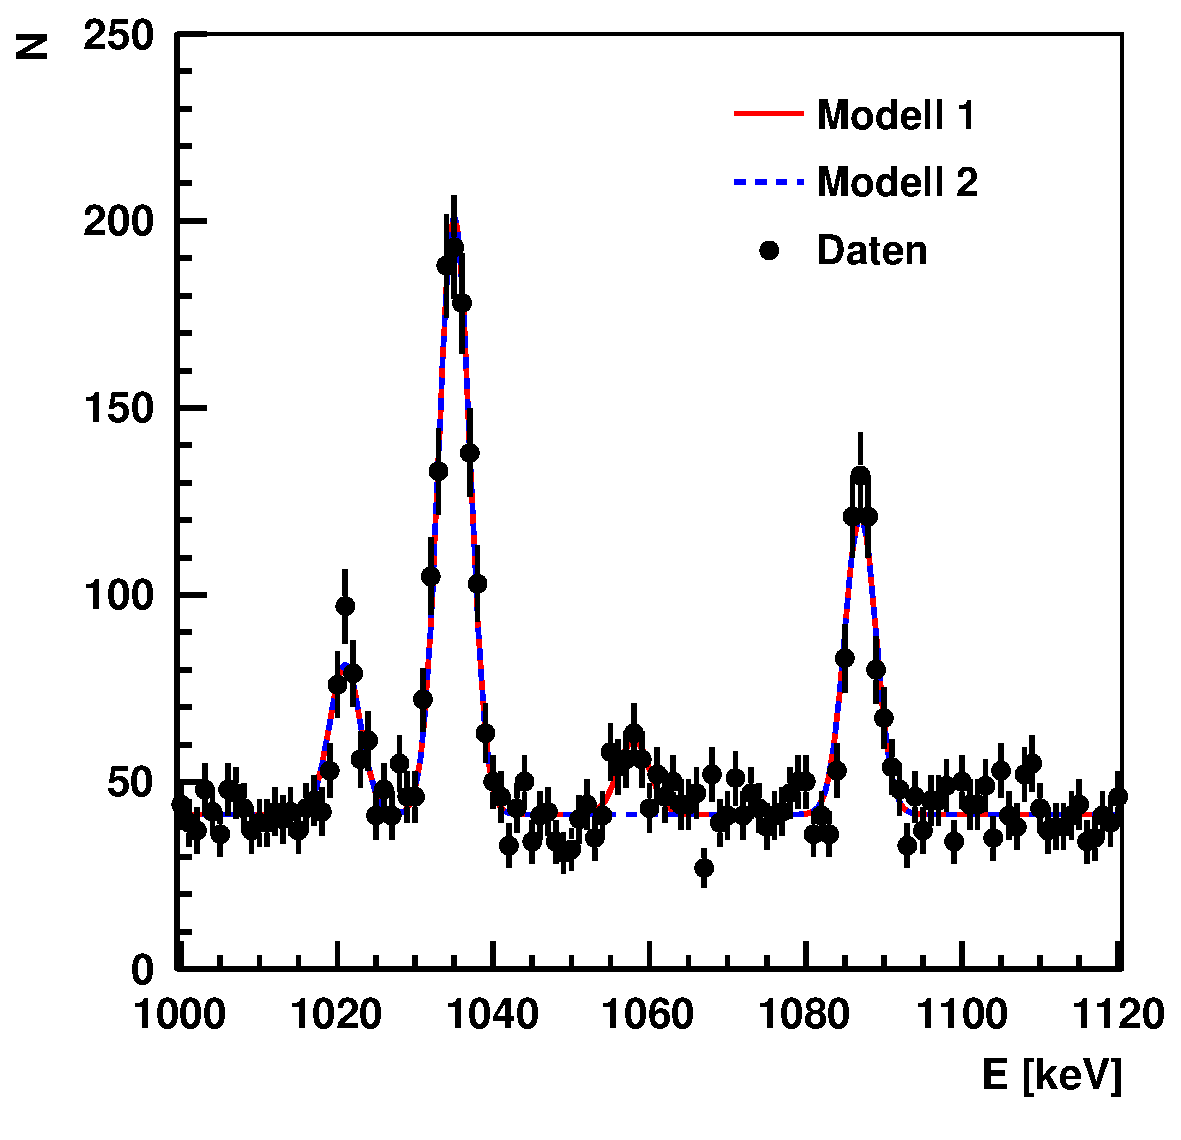
\includegraphics[width=0.5\textwidth]{plot.pdf}
%    \caption{A figure caption~\cite{brandt}.}
%    \label{fig:fig1}
%  \end{center}
%\end{figure}
